\begin{figure}[h]
	\centering
	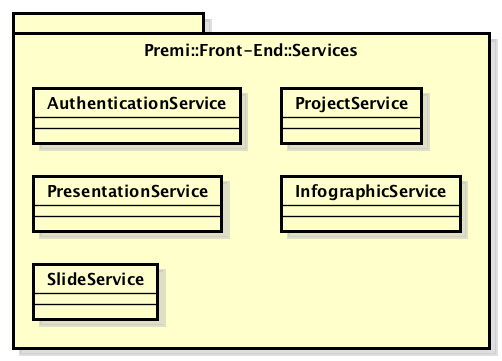
\includegraphics[width=0.7\linewidth]{img/premi_front_end_services}
	\caption[Premi::Front-End::Services]{Premi::Front-End::Services}
\end{figure}
Il package gestisce i services del \gls{front-end} dell'applicazione. Comunica con i controller e con i servizi \gls{REST} offerti dal lato \gls{back-end}, fornendo delle risorse sulle quali creare le funzioni per comunicare tra i due layer. La struttura prevede cinque service principali i quali al loro interno contengono dei metodi specifici che forniscono le risorse per dei servizi più precisi.
Per brevità nell'identificare un service è stata omessa la dicitura Premi::\gls{Front-End}::Services lasciando solamente il nome del service stesso. Si assume dunque che la dicitura compatta <nomeService> rappresenta la forma estesa Premi::\gls{Front-End}::Services::<nomeService>.
\newpage


\subsubsection{AuthenticationService}
L'AuthenticationService è una classe che fornisce ulteriori metodi per gestire le funzioni di autenticazione al sito e di gestione degli utenti. Mette a disposizione ulteriori servizi con il compito di creare delle risorse utilizzabili dai metodi creati nei controller per la gestione del login, logout e della registrazione, la gestione dei dati utente e il recupero delle credenziali.

		\subsubsection{AuthenticationService::forgotPasswordService}
		\begin{figure}[h]
			\centering
				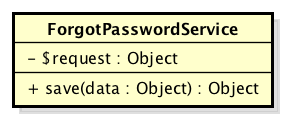
\includegraphics[width=0.4\linewidth]{img/premi_front_end_services_forgotpasswordservice}
			\caption[Premi::Front-End::Services::ForgotPasswordService]{Premi::Front-End::Services::ForgotPasswordService}
		\end{figure}
		
		\paragraph{Descrizione}
		Si occupa di gestire il processo di recupero password per l'autenticazione dell'utente.
		
		\paragraph{Utilizzo}
		Viene utilizzato per creare una risorsa collegata al servizio \gls{REST} che permette il recupero della password dell'utente.
		
		\paragraph{Relazioni con le altre classi}
		\begin{itemize}
			\item OUT: \textbf{AuthenticationCtrl}:\\
			Classe che gestisce le operazioni per l'autenticazione dell'utente al sistema.
		\end{itemize}
		
		\paragraph{Attributi}
		\begin{itemize}
			\item \textbf{- \$request: Object}:\\
			Campo dati contenente la route per la chiamata al servizio \gls{REST} specifico del servizio.
		\end{itemize}	
		
		\paragraph{Metodi}
		\begin{itemize}
			\item \textbf{+ save(data: Object)}:\\
			Metodo che richiama la funzione PUT collegata alla risorsa e permette di eseguire la chiamata alla funzione definita nella parte di backend la quale avvia il processo di recupero password, inviando una mail all'indirizzo passato attraverso il parametro della funzione.\\
			\textbf{Parametri:}\\
			\begin{itemize}
				\item \textit{data: Object}: parametro di un oggetto \gls{JSON} che contiene l'indirizzo email inserito nella view.
			\end{itemize}
		\end{itemize}
\newpage
		
		
		\subsubsection{AuthenticationService::loginService}
		\begin{figure}[h]
			\centering
				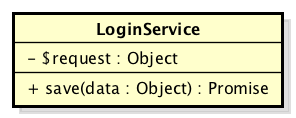
\includegraphics[width=0.4\linewidth]{img/premi_front_end_services_loginservice}
			\caption[Premi::Front-End::Services::LoginService]{Premi::Front-End::Services::LoginService}
		\end{figure}
		
		\paragraph{Descrizione}
		Si occupa di gestire il processo di login dell'utente.
		
		\paragraph{Utilizzo}
		Viene utilizzato per creare una risorsa collegata al servizio \gls{REST} che permette l'autenticazione dell'utente al sistema.
		
		\paragraph{Relazioni con le altre classi}
		\begin{itemize}
			\item OUT: \textbf{AuthenticationCtrl}:\\
			Classe che gestisce le operazioni per l'autenticazione dell'utente al sistema.
		\end{itemize}
		
		\paragraph{Attributi}
		\begin{itemize}
			\item \textbf{- \$request: Object}:\\
			Campo dati contenente la route per la chiamata al servizio \gls{REST} specifico del servizio.
		\end{itemize}	
		
		\paragraph{Metodi}
		\begin{itemize}
			\item \textbf{+ save(data: Object): Promise}:\\
			Metodo che richiama la funzione PUT collegata alla risorsa e permette di eseguire il login dell'utente al sistema. Il metodo ritorna una promessa la quale, se ha esito positivo, verrà analizzata per ottenere lo username dell'utente o il messaggio di errore. \\
			\textbf{Parametri:}\\
			\begin{itemize}
				\item \textit{data: Object}: parametro di un oggetto \gls{JSON} che contiene il nome utente e la password inseriti nella view e necessari per l'autenticazione al sistema.
			\end{itemize}
		\end{itemize}
\newpage
		
		
		\subsubsection{AuthenticationService::logoutService}
		\begin{figure}[h]
			\centering
				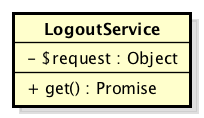
\includegraphics[width=0.4\linewidth]{img/premi_front_end_services_logoutservice}
			\caption[Premi::Front-End::Services::LogoutService]{Premi::Front-End::Services::LogoutService}
		\end{figure}
		
		\paragraph{Descrizione}
		Si occupa di gestire il processo di logout dell'utente.
		
		\paragraph{Utilizzo}
		Viene utilizzato per creare una risorsa collegata al servizio \gls{REST} che permette l'autenticazione dell'utente al sistema.
		
		\paragraph{Relazioni con le altre classi}
		\begin{itemize}
			\item OUT: \textbf{AuthenticationCtrl}:\\
			Classe che gestisce le operazioni per l'autenticazione dell'utente al sistema.
		\end{itemize}
		
		\paragraph{Attributi}
		\begin{itemize}
			\item \textbf{- \$request: Object}:\\
			Campo dati contenente la route per la chiamata al servizio \gls{REST} specifico del servizio.
		\end{itemize}	
		
		\paragraph{Metodi}
		\begin{itemize}
			\item \textbf{+ get(): Promise}:\\
			Metodo che richiama la funzione GET collegata alla risorsa e permette di eseguire il logout dell'utente. Il metodo ritorna una promessa e porta all'aggiornamento della pagina per il reset delle variabili si \$scope.
		\end{itemize}
\newpage
		
		
		\subsubsection{AuthenticationService::signUpService}
		\begin{figure}[h]
			\centering
				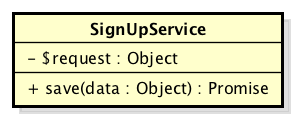
\includegraphics[width=0.4\linewidth]{img/premi_front_end_services_signupservice}
			\caption[Premi::Front-End::Services::SignupService]{Premi::Front-End::Services::SignupService}
		\end{figure}
		
		\paragraph{Descrizione}
		Si occupa di gestire il processo di registrazione dell'utente.
		
		\paragraph{Utilizzo}
		Viene utilizzato per creare una risorsa collegata al servizio \gls{REST} che permette l'autenticazione dell'utente al sistema.
		
		\paragraph{Relazioni con le altre classi}
		\begin{itemize}
			\item OUT: \textbf{AuthenticationCtrl}:\\
			Classe che gestisce le operazioni per l'autenticazione dell'utente al sistema.
		\end{itemize}
		
		\paragraph{Attributi}
		\begin{itemize}
			\item \textbf{- \$request: Object}:\\
			Campo dati contenente la route per la chiamata al servizio \gls{REST} specifico del servizio.
		\end{itemize}	
		
		\paragraph{Metodi}
		\begin{itemize}
			\item \textbf{+ save(data: Object): Promise}:\\
			Metodo che richiama la funzione PUT collegata alla risorsa e permette di eseguire la registrazione dell'utente al sistema. Il metodo ritorna una promessa la quale, se la chiamata ha esito positivo, verrà analizzata per ottenere la conferma di avvenuta registrazione o altrimenti, l'array contenenti gli errori commessi nell'inserimento dei dati.\\
			\textbf{Parametri:}\\
			\begin{itemize}
				\item \textit{data: Object}: parametro di un oggetto \gls{JSON} che contiene tutte le credenziali necessarie inserite nella view per registrarsi come nuovo utente al sistema.
			\end{itemize}
		\end{itemize}
\newpage
		
		
		\subsubsection{AuthenticationService::userService}
		\begin{figure}[h]
			\centering
				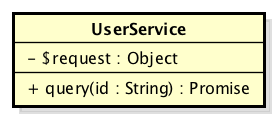
\includegraphics[width=0.4\linewidth]{img/premi_front_end_services_userservice}
			\caption[Premi::Front-End::Services::UserService]{Premi::Front-End::Services::UserService}
		\end{figure}
		
		\paragraph{Descrizione}
		Si occupa di gestire le operazioni riguardanti un utente.
		
		\paragraph{Utilizzo}
		Viene utilizzato per creare una risorsa collegata al servizio \gls{REST} che permette di gestire le operazioni riguardanti un utente, quali il recupero dei suoi dati.
		
		\paragraph{Relazioni con le altre classi}
		\begin{itemize}
			\item OUT: \textbf{MyAccountCtrl}:\\
			Classe che gestisce la rappresentazione dei dati di un utente.
		\end{itemize}
		
		\paragraph{Attributi}
		\begin{itemize}
			\item \textbf{- \$request: Object}:\\
			Campo dati contenente la route per la chiamata al servizio \gls{REST} specifico del servizio.
		\end{itemize}	
		
		\paragraph{Metodi}
		\begin{itemize}
			\item \textbf{+ query(id:String): Promise}:\\
			Metodo che richiama la funzione GET collegata alla risorsa e permette di ottenere i dati relativi all'utente con id passato come parametro. Il metodo ritorna una promessa contenete tutti i dati dell'utente
			\textbf{Parametri:}\\
			\begin{itemize}
				\item \textit{id: String}: parametro di una stringa contenente l'id dell'utente.
			\end{itemize}
		\end{itemize}
\newpage


\subsubsection{InfographicService}
L'InfographicService è una classe che mette a disposizione dei metodi per la gestione delle infografiche di un progetto. Con questi metodi è possibile creare delle risorse con le quali si possono creare, modificare o eliminare delle infografiche.

		
		\subsubsection{InfographicService::infographicEditorService}
		\begin{figure}[h]
			\centering
				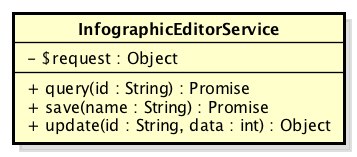
\includegraphics[width=0.4\linewidth]{img/premi_front_end_services_infographiceditorservice}
			\caption[Premi::Front-End::Services::InfographicEditorService]{Premi::Front-End::Services::infographicEditorService}
		\end{figure}
		
		\paragraph{Descrizione}
		Si occupa di gestire le operazioni riguardanti le infografiche del progetto.
		
		\paragraph{Utilizzo}
		Viene utilizzato per creare una risorsa collegata al servizio \gls{REST} che permette di gestire le operazioni sulle infografiche, quali la crezione, la modifica, il salvataggio e l'eliminazione.
		
		\paragraph{Relazioni con le altre classi}
		\begin{itemize}
			\item OUT: \textbf{InfographicEditorCtrl}:\\
			Classe che gestisce le operazioni di modifica di una \gls{infografica}.
		\end{itemize}
		
		\paragraph{Attributi}
		\begin{itemize}
			\item \textbf{- \$request: Object}:\\
			Campo dati contenente la route per la chiamata al servizio \gls{REST} specifico del servizio.
		\end{itemize}	
		
		\paragraph{Metodi}
		\begin{itemize}
			\item \textbf{+ query(id: String): Promise}:\\
				Metodo che richiama la funzione GET collegata alla risorsa e permette di caricare l'\gls{infografica} richiesta dal \gls{database}. Il metodo ritorna una promessa la quale, se la chiamata ha esito positivo, conterrà l'\gls{infografica} con tutti i propri dati.\\
			\item \textbf{+ save(name: String): Promise}:\\
				Metodo che richiama la funzione POST collegata alla risorsa e permette di creare una nuova \gls{infografica} e di salvarla nel \gls{database}. Il metodo ritorna una promessa la quale, se la chiamata ha esito positivo, conterrà il valore \textit{true}.\\
			\item \textbf{+ update(id: String, data:Object): Promise}:\\
				Metodo che richiama la funzione PUT collegata alla risorsa e permette di salvare l'\gls{infografica} aggiornando i dati passati per parametro. Il metodo ritorna una promessa la quale, se la chiamata ha esito positivo, conterrà il valore \textit{true}.\\
			\textbf{Parametri:}\\
			\begin{itemize}
				\item \textit{id: String}: parametro di una stringa contenente l'id dell'\gls{infografica} sulla quale eseguire le operazioni;
				\item \textit{name: String}: parametro di una stringa contenente il nome dell'\gls{infografica} da creare;
				\item \textit{data: Object}: parametro di una oggetto contenente i dati necessari per aggiornare l'\gls{infografica}.
			\end{itemize}
		\end{itemize}
\newpage


\subsubsection{PresentationService}
Il PresentationService rende disponibili dei servizi che si occupano della gestione di una presentazione. Con le risorse che si possono creare, è possibile visualizzare una presentazione oppure modificarla attraverso le opportune chiamate eseguite nella sezione dell'editor.


		\subsubsection{PresentationService::presentationService}
		\begin{figure}[h]
			\centering
				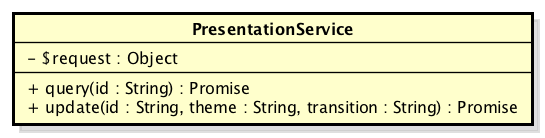
\includegraphics[width=0.5\linewidth]{img/premi_front_end_services_presentationservice}
			\caption[Premi::Front-End::Services::PresentationService]{Premi::Front-End::Services::PresentationService}
		\end{figure}
		
		\paragraph{Descrizione}
		Si occupa di gestire le operazioni riguardanti la presentazione di un progetto.
		
		\paragraph{Utilizzo}
		Viene utilizzato per creare una risorsa collegata al servizio \gls{REST} che permette di gestire le operazioni sulle presentazioni, cioè di caricarle dal backend oppure di salvarle nel \gls{database}.
		
		\paragraph{Relazioni con le altre classi}
		\begin{itemize}
			\item OUT: \textbf{PresentationCtrl}:\\
			Classe che gestisce le operazioni di visualizzazione di una presentazione;
			\item OUT: \textbf{PresentationEditorCtrl}:\\
			Classe che gestisce le operazioni modifica di una presentazione;
			\item OUT: \textbf{SlideEditorCtrl}:\\
			Classe che gestisce le operazioni di modifica di una \gls{slide}.
		\end{itemize}
		
		\paragraph{Attributi}
		\begin{itemize}
			\item \textbf{- \$request: Object}:\\
			Campo dati contenente la route per la chiamata al servizio \gls{REST} specifico del servizio.
		\end{itemize}	
		
		\paragraph{Metodi}
		\begin{itemize}
			\item \textbf{+ query(id: String): Promise}:\\
			Metodo che richiama la funzione GET collegata alla risorsa e permette di caricare la presentazione dal \gls{database}. Il metodo ritorna una promessa la quale, se la chiamata ha esito positivo, conterrà la presentazione con tutte le rispettive \gls{slide}.\\
			\item \textbf{+ update(id: String, theme:String, transition:String): Promise}:\\
			Metodo che richiama la funzione POST collegata alla risorsa e permette di salvare la presentazione aggiornando i dati, anche quelli riguardanti il tema e la transizione tra le \gls{slide} passati per parametro. Il metodo ritorna una promessa la quale, se la chiamata ha esito positivo, conterrà il valore \textit{true}.\\
			\textbf{Parametri:}\\
			\begin{itemize}
				\item \textit{id: String}: parametro di una stringa contenente l'id della presentazione sulla quale eseguire le operazioni;
				\item \textit{theme: String}: parametro di una stringa contenente il nome del tema da applicare alla presentazione;
				\item \textit{transition: String}: parametro di una stringa contenente il nome della transizione da applicare alla presentazione.
			\end{itemize}
		\end{itemize}
\newpage


\subsubsection{ProjectService}
ProjectService è una classe che mette a disposizione i metodi per l'organizzazione di un progetto. Con le risorse create da questi, è possibile caricare e salvare un progetto già presente nel \gls{database}, eliminarlo oppure crearne uno di nuovo inserendo i parametri opportuni.

		\subsubsection{ProjectService::projectsService}
		\begin{figure}[h]
			\centering
				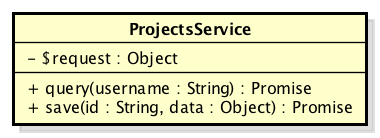
\includegraphics[width=0.4\linewidth]{img/premi_front_end_services_projectsservice}
			\caption[Premi::Front-End::Services::ProjectsService]{Premi::Front-End::Services::ProjectsService}
		\end{figure}
		
		\paragraph{Descrizione}
		Si occupa di gestire le operazioni riguardanti i progetti.
		
		\paragraph{Utilizzo}
		Viene utilizzato per creare una risorsa collegata al servizio \gls{REST} che permette di gestire le operazioni sui progetti, cioè di caricarli o eliminarli dal \gls{database}.
		
		\paragraph{Relazioni con le altre classi}
		\begin{itemize}
			\item OUT: \textbf{MyProjectsCtrl}:\\
			Classe che gestisce le operazioni riguardanti i progetti personali di un utente;
			\item OUT: \textbf{ProjectCtrl}:\\
			Classe che gestisce le operazioni riguardanti i progetti;
			\item OUT: \textbf{SearchCtrl}:\\
			Classe che gestisce le operazioni di ricerca. Viene usato per caricare i progetti trovati.
		\end{itemize}
		
		\paragraph{Attributi}
		\begin{itemize}
			\item \textbf{- \$request: Object}:\\
			Campo dati contenente la route per la chiamata al servizio \gls{REST} specifico del servizio.
		\end{itemize}	
		
		\paragraph{Metodi}
		\begin{itemize}
			\item \textbf{+ query(username: String): Promise}:\\
			Metodo che richiama la funzione GET collegata alla risorsa e permette di caricare i progetti dell'utente con username passato per parametro e i rispettivi contenuti dal \gls{database}. Il metodo ritorna una promessa la quale, se la chiamata ha esito positivo, conterrà un oggetto avente il progetto e i suoi dati.\\
			\item \textbf{+ save(id: String, data:Object): Promise}:\\
			Metodo che richiama la funzione POST collegata alla risorsa e permette di creare un nuovo progetto con i dati passati per parametro. Il metodo ritorna una promessa la quale, se la chiamata ha esito positivo, conterrà il valore \textit{true}.\\
			\textbf{Parametri:}\\
			\begin{itemize}
				\item \textit{username: String}: parametro di una stringa contenente lo username dell'utente;
				\item \textit{id: String}: parametro di una stringa contenente l'id del progetto sul quale eseguire le operazioni;
				\item \textit{data: Object}: parametro di un oggetto contenente i dati necessari per creare il progetto, quali ad esempio il nome.
			\end{itemize}
		\end{itemize}
\newpage
		
		
		\subsubsection{ProjectService::searchByProjectService}
		\begin{figure}[h]
			\centering
				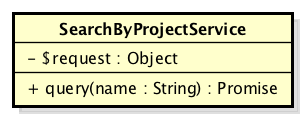
\includegraphics[width=0.4\linewidth]{img/premi_front_end_services_searchbyprojectservice}
			\caption[Premi::Front-End::Services::SearchByProjectService]{Premi::Front-End::Services::SearchByProjectService}
		\end{figure}
		
		\paragraph{Descrizione}
		Si occupa di gestire il processo di ricerca del sistema.
		
		\paragraph{Utilizzo}
		Viene utilizzato per creare una risorsa collegata al servizio \gls{REST} che permette la ricerca nel sistema attraverso il nome del progetto.
		
		\paragraph{Relazioni con le altre classi}
		\begin{itemize}
			\item OUT: \textbf{HomePageCtrl}:\\
			Classe che gestisce le operazioni di reindirizzamento tra le pagine dall'applicazione e le operazioni di ricerca.
		\end{itemize}
		
		\paragraph{Attributi}
		\begin{itemize}
			\item \textbf{- \$request: Object}:\\
			Campo dati contenente la route per la chiamata al servizio \gls{REST} specifico del servizio.
		\end{itemize}	
		
		\paragraph{Metodi}
		\begin{itemize}
			\item \textbf{+ query(name: String): Promise}:\\
			Metodo che richiama la funzione GET collegata alla risorsa e permette di eseguire la ricerca nel sistema attraverso il nome di un progetto. Il metodo ritorna una promessa la quale, se la chiamata ha esito positivo, conterrà un array con i dati relativi ai progetti risultato della ricerca.\\
			\textbf{Parametri:}\\
			\begin{itemize}
				\item \textit{name: String}: parametro di una stringa contenente il nome del progetto da cercare inserito nella view.
			\end{itemize}
		\end{itemize}
\newpage
		
		
		\subsubsection{ProjectService::searchByUserService}
		\begin{figure}[h]
			\centering
				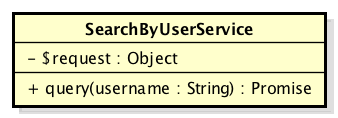
\includegraphics[width=0.4\linewidth]{img/premi_front_end_services_searchbyuserservice}
			\caption[Premi::Front-End::Services::SearchByUserService]{Premi::Front-End::Services::SearchByUserService}
		\end{figure}
		
		\paragraph{Descrizione}
		Si occupa di gestire il processo di ricerca del sistema.
		
		\paragraph{Utilizzo}
		Viene utilizzato per creare una risorsa collegata al servizio \gls{REST} che permette la ricerca nel sistema attraverso il nome utente.
		
		\paragraph{Relazioni con le altre classi}
		\begin{itemize}
			\item OUT: \textbf{HomePageCtrl}:\\
			Classe che gestisce le operazioni di reindirizzamento tra le pagine dall'applicazione e le operazioni di ricerca.
		\end{itemize}
		
		\paragraph{Attributi}
		\begin{itemize}
			\item \textbf{- \$request: Object}:\\
			Campo dati contenente la route per la chiamata al servizio \gls{REST} specifico del servizio.
		\end{itemize}	
		
		\paragraph{Metodi}
		\begin{itemize}
			\item \textbf{+ query(username: String): Promise}:\\
			Metodo che richiama la funzione GET collegata alla risorsa e permette di eseguire la ricerca nel sistema attraverso lo username di un utente. Il metodo ritorna una promessa la quale, se la chiamata ha esito positivo, conterrà un array con gli utenti risultato della ricerca, ognuno dei quali avrà le informazioni necessarie per recuperare i rispettivi progetti da analizzare.\\
			\textbf{Parametri:}\\
			\begin{itemize}
				\item \textit{username: String}: parametro di una stringa contenente il nome utente da cercare inserito nella view.
			\end{itemize}
		\end{itemize}
\newpage
		
		
		\subsubsection{ProjectService::projectService}
		\begin{figure}[h]
			\centering
				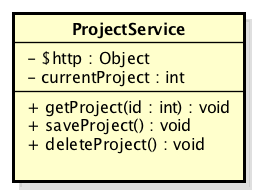
\includegraphics[width=0.4\linewidth]{img/premi_front_end_services_projectservice}
			\caption[Premi::Front-End::Services::ProjectService]{Premi::Front-End::Services::ProjectService}
		\end{figure}
		
		\paragraph{Descrizione}
		Si occupa di gestire le operazioni riguardanti uno specifico progetto di un utente.
		
		\paragraph{Utilizzo}
		Viene utilizzato per creare una risorsa collegata al servizio \gls{REST} che permette di gestire le operazioni sul progetto, cioè di caricarlo o eliminarli dal \gls{database}.
		
		\paragraph{Relazioni con le altre classi}
		\begin{itemize}
			\item OUT: \textbf{ProjectCtrl}:\\
				Classe che gestisce le operazioni riguardanti i progetti;
			\item OUT: \textbf{HomeCtrl}:\\
				Classe che gestisce le operazioni riguardanti la home page del sito.
		\end{itemize}
		
		\paragraph{Attributi}
		\begin{itemize}
			\item \textbf{- \$request: Object}:\\
			Campo dati contenente la route per la chiamata al servizio \gls{REST} specifico del servizio.
		\end{itemize}	
		
		\paragraph{Metodi}
		\begin{itemize}
			\item \textbf{+ delete(id: String): Promise}:\\
			Metodo che richiama la funzione DELETE collegata alla risorsa e permette di rimuovere il progetto e tutto il suo contenuto dal \gls{database}. Il metodo ritorna una promessa la quale, se la chiamata ha esito positivo, conterrà il valore \textit{true}.\\
			\item \textbf{+ update(id: String, data:Object): Promise}:\\
			Metodo che richiama la funzione PUT collegata alla risorsa e permette di aggiornare i dati del progetto passati per parametro. Il metodo ritorna una promessa la quale, se la chiamata ha esito positivo, conterrà il valore \textit{true}.\\
			\textbf{Parametri:}\\
			\begin{itemize}
				\item \textit{id: String}: parametro di una stringa contenente l'id del progetto sul quale eseguire le operazioni;
				\item \textit{data: Object}: parametro di un oggetto contenente i dati del progetto da aggiornare.
			\end{itemize}
		\end{itemize}
\newpage


\subsubsection{SlideService}
SlideService è l'ultimo dei macro servizi offerti e si occupa della gestione delle \gls{slide} che compongono una presentazione. Con i metodi che mette a disposizione vengono create delle risorse apposite adatte a gestire tutte le operazioni che è possibile eseguire in una \gls{slide}.


		\subsubsection{SlideService::indexService}
		\begin{figure}[h]
			\centering
				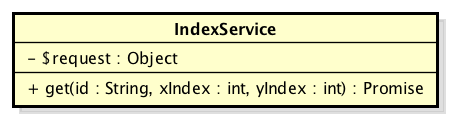
\includegraphics[width=0.4\linewidth]{img/premi_front_end_services_indexservice}
			\caption[Premi::Front-End::Services::IndexService]{Premi::Front-End::Services::IndexService}
		\end{figure}
		
		\paragraph{Descrizione}
		Si occupa di gestire le operazioni riguardanti gli indici delle \gls{slide}.
		
		\paragraph{Utilizzo}
		Viene utilizzato per creare una risorsa collegata al servizio \gls{REST} che permette di gestire le operazioni riguardanti gli indici delle \gls{slide}.
		
		\paragraph{Relazioni con le altre classi}
		\begin{itemize}
			\item OUT: \textbf{SlideServiceCtrl}:\\
			Classe che gestisce le operazioni riguardanti le \gls{slide} di un progetto.
		\end{itemize}
		
		\paragraph{Attributi}
		\begin{itemize}
			\item \textbf{- \$request: Object}:\\
			Campo dati contenente la route per la chiamata al servizio \gls{REST} specifico del servizio.
		\end{itemize}	
		
		\paragraph{Metodi}
		\begin{itemize}
			\item \textbf{+ get(id: String, xIndex:int, yIndex:int): Promise}:\\
			Metodo che richiama la funzione GET collegata alla risorsa e permette di ottenere la \gls{slide} avente x e y corrispondenti ai parametri passati. Il metodo ritorna una promessa la quale, se la chiamata ha esito positivo, conterrà un oggetto avente l'id della \gls{slide}.\\
			\textbf{Parametri:}\\
			\begin{itemize}
				\item \textit{id: String}: parametro di una stringa contenente l'id del progetto sul quale eseguire la funzione;
				\item \textit{xIndex: int}: parametro di un intero rappresentate la coordinata x della \gls{slide} richiesta;
				\item \textit{yIndex: int}: parametro di un intero rappresentate la coordinata y della \gls{slide} richiesta.
			\end{itemize}
		\end{itemize}
\newpage
		
		\subsubsection{SlideService::slideService}
		\begin{figure}[h]
			\centering
				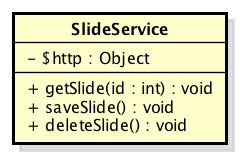
\includegraphics[width=0.5\linewidth]{img/premi_front_end_services_slideservice}
			\caption[Premi::Front-End::Services::SlideService]{Premi::Front-End::Services::SlideService}
		\end{figure}
		
		\paragraph{Descrizione}
		Si occupa di gestire le operazioni di una \gls{slide}.
		
		\paragraph{Utilizzo}
		Viene utilizzato per creare una risorsa collegata al servizio \gls{REST} che permette di modificare una \gls{slide}. Dà la possiblità di creare, caricare, salvare e eliminare una \gls{slide} dal \gls{database}.
		
		\paragraph{Relazioni con le altre classi}
		\begin{itemize}
			\item OUT: \textbf{SlideEditorCtrl}:\\
			Classe che gestisce le operazioni di modifica di una \gls{slide}.
		\end{itemize}
		
		\paragraph{Attributi}
		\begin{itemize}
			\item \textbf{- \$request: Object}:\\
			Campo dati contenente la route per la chiamata al servizio \gls{REST} specifico del servizio.
		\end{itemize}	
		
		\paragraph{Metodi}
		\begin{itemize}
			\item \textbf{+ get(id:String): Promise}:\\
			Metodo che richiama la funzione GET collegata alla risorsa e permette di ottenere la \gls{slide} dal backend identificata dall'id passato come parametro. IL metodo ritorna una promessa contenente un oggetto \gls{JSON} avente tutte le informazioni e i dati riguardanti la \gls{slide} e i suoi componenti. Questo oggetto è pronto per essere passato all'apposito metodo di caricamento della \gls{slide};
			\item \textbf{+ save(xIndex:int, yIndex:int): Promise}:\\
			Metodo che richiama la funzione POST collegata alla risorsa e permette di creare una nuova \gls{slide} avente le coordinate passate per parametro. Il metodo ritorna una promessa la quale, se la chiamata ha esito positivo, conterrà l'id della nuova \gls{slide} creata;\\
			\item \textbf{+ update(id:String, xIndex:int, yIndex:int, components:JSON, background:String, slideSVG:SVG):Promise}\\
			Metodo che richiama la funzione PUT collegata alla risorsa e permette di aggiornare una \gls{slide} già creata (identificata dal parametro id). Con questa chiamata è possibile passare le coordinate aggiornate, i componenti della \gls{slide}, il colore di sfondo e l'SVG rappresentante la \gls{slide} stessa. Il metodo ritorna una promessa che conterrà \textit{true} se l'esito del salvataggio è positivo;
			\item \textbf{+ delete(id:String):Promise}\\
			Metodo che richiama la funzione DELETE collegata alla risorsa e permette di eliminare la \gls{slide} con id passato per parametro. Il metodo ritorna una promessa che conterrà \textit{true} se l'esito del salvataggio è positivo.
			
			\textbf{Parametri:}\\
			\begin{itemize}
				\item \textit{background: String}: parametro di una stringa che contiene il codice del colore di sfondo della \gls{slide};
				\item \textit{components: JSON}: parametro di un oggetto \gls{JSON} contenente tutti i componenti inclusi nella \gls{slide};
				\item \textit{id: String}: parametro di una stringa contenente l'id del progetto sul quale eseguire la funzione;
				\item \textit{slideSVG: SVG}: parametro di un oggetto SVG che contiene la rappresentazione della \gls{slide} in SVG;
				\item \textit{xIndex: int}: parametro di un intero rappresentate la coordinata x della \gls{slide} richiesta;
				\item \textit{yIndex: int}: parametro di un intero rappresentate la coordinata y della \gls{slide} richiesta.
			\end{itemize}
		\end{itemize}
\newpage		
		
\subsubsection{SlideService::componentService}
	\begin{figure}[h]
		\centering
		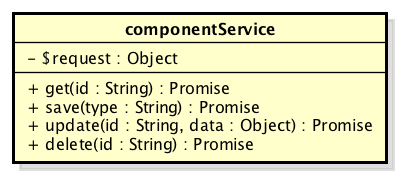
\includegraphics[width=0.5\linewidth]{img/premi_front_end_services_componentservice}
		\caption[Premi::Front-End::Services::ComponentService]{Premi::Front-End::Services::ComponentService}
	\end{figure}
	
	\paragraph{Descrizione}
	Si occupa di gestire le operazioni dei componenti di una \gls{slide}.
	
	\paragraph{Utilizzo}
	Viene utilizzato per creare una risorsa collegata al servizio \gls{REST} che permette di modificare un componente di una \gls{slide}.
	
	\paragraph{Relazioni con le altre classi}
	\begin{itemize}
		\item OUT: \textbf{ChartCtrl}:\\
			Classe che gestisce le operazioni di modifica di un componente di tipo grafico;
		\item OUT: \textbf{ImageCtrl}:\\
			Classe che gestisce le operazioni di modifica di un componente di tipo immagine;
		\item OUT: \textbf{RealTimeDataCtrl}:\\
			Classe che gestisce le operazioni di modifica di un componente di tipo dato realtime;
		\item OUT: \textbf{TableCtrl}:\\
			Classe che gestisce le operazioni di modifica di un componente di tipo tabella;
		\item OUT: \textbf{TextCtrl}:\\
			Classe che gestisce le operazioni di modifica di un componente di tipo grafico.
	\end{itemize}
	
	\paragraph{Attributi}
	\begin{itemize}
		\item \textbf{- \$request: Object}:\\
		Campo dati contenente la route per la chiamata al servizio \gls{REST} specifico del servizio.
	\end{itemize}	
	
	\paragraph{Metodi}
	\begin{itemize}
		\item \textbf{+ get(id:String): Promise}:\\
			Metodo che richiama la funzione GET collegata alla risorsa e permette di ottenere il componente richiesto. Il metodo ritorna una promessa che conterrà i dati del componente.
		\item \textbf{+ save(type:String): Promise}:\\
			Metodo che richiama la funzione POST collegata alla risorsa e permette di creare un nuovo componente del tipo richiesto attraverso il parametro. Il metodo ritorna una promessa la quale, se la chiamata ha esito positivo, conterrà l'id della nuova \gls{slide} creata;\\
		\item \textbf{+ update(id:String, data:Object):Promise}\\
			Metodo che richiama la funzione PUT collegata alla risorsa e permette di aggiornare un componente già creato in precedenza con i dati passi per parametro. Il metodo ritorna una promessa che conterrà il valore \textit{true} se il processo è andato a buon fine. 
		\item \textbf{+ delete(id:String):Promise}\\
			Metodo che richiama la funzione DELETE collegata alla risorsa e permette di eliminare il componente con id passato per parametro. Il metodo ritorna una promessa che conterrà \textit{true} se l'esito del salvataggio è positivo.
		
		\textbf{Parametri:}\\
		\begin{itemize}
			\item \textit{id: String}: parametro di una stringa contenente l'id del componente sul quale eseguire la funzione;
			\item \textit{type: String}: parametro di un oggetto di tipo stringa che contiene il tipo di componente da creare;
			\item \textit{data: Object}: parametro di un oggetto contente le informazioni sul componente da salvare.
		\end{itemize}
	\end{itemize}
